\documentclass[]{article}
\usepackage[]{graphicx}
\usepackage[]{xcolor}

\begin{document}
\author{Matteo Ielacqua}
\title{Github Social}
\maketitle
    \section{Brief introduction}
    A large social network of GitHub developers which was collected from the public API in June 2019. Nodes are developers who have starred at least 10 repositories and edges are mutual follower relationships between them.
    \subsection*{Context}
    GitHub is a double scope platform: In first place is used to store and develop software , either by open source developers and by companies, secondly is a social network for developers in which them can argue about technical solution and future projects. In GitHub a user can Fork ( copy the repository in his own userspace), view the code and star a repository. The star operation is a follow operation, thus a user can track the progress on certain repository. But is also possible to follow a developer to see which project he taken part to, and that's what the network is collecting. 
    \subsection*{What to expect}
    This is a social network, so we expect a sparse graph with very few node very popular and most of them not. Most of the nodes should be part of a giant component. Triadic closure is probably given by some developers working on the same project (assumpting that the node is respecting the requirements of have starred 10 repositiories) and so we expect the presence of some big communities given by the presence of big project (like for example Unreal Engine source code or Qt company code).  

    \section*{Communities}
    Using PLM (Parallel Louvain) as community detection algorithm, the subsequent values are found:
    \begin{itemize}
        \item Modularity: 0.452411
        \item Partitions: 28
        \item Element in partitions: 37700
        \item Size min: 3
        \item Size max: 7654
        \item Size Mean: 1346.43   
    \end{itemize}
    The algorithm detected 28 sub partitions and the maximum modularity is near 0.5, that could be mean that in general nodes tend to form link also outside the communities. That is very likely due to the context, in fact developers that are working on the same project in order to monitor commits on the same project tend to follow their colleague, but nobody said that a developer would work only on a single project, hovewer the cause of a poor modularity could be the algorithm itself, so a new run using label propagation could be required.
    
    \begin{itemize}
        \item Modularity: 0.000200665
        \item Partitions: 11
        \item Element in partitions: 37700
        \item Size min: 3
        \item Size max: 37658
        \item Size Mean: 3427.27
    \end{itemize}

    Totally different result came up. Hovewer label propagation is confirming the hypothesis done before, developers tend to follow other developers outside projects. The very low modularity (near 0 this time) could indicate that this phenomenon is much like than expected. Let's see something about sizes, Louvain and Label propagation found 2 different result, but similiar in some way.\\
    \colorbox{black}{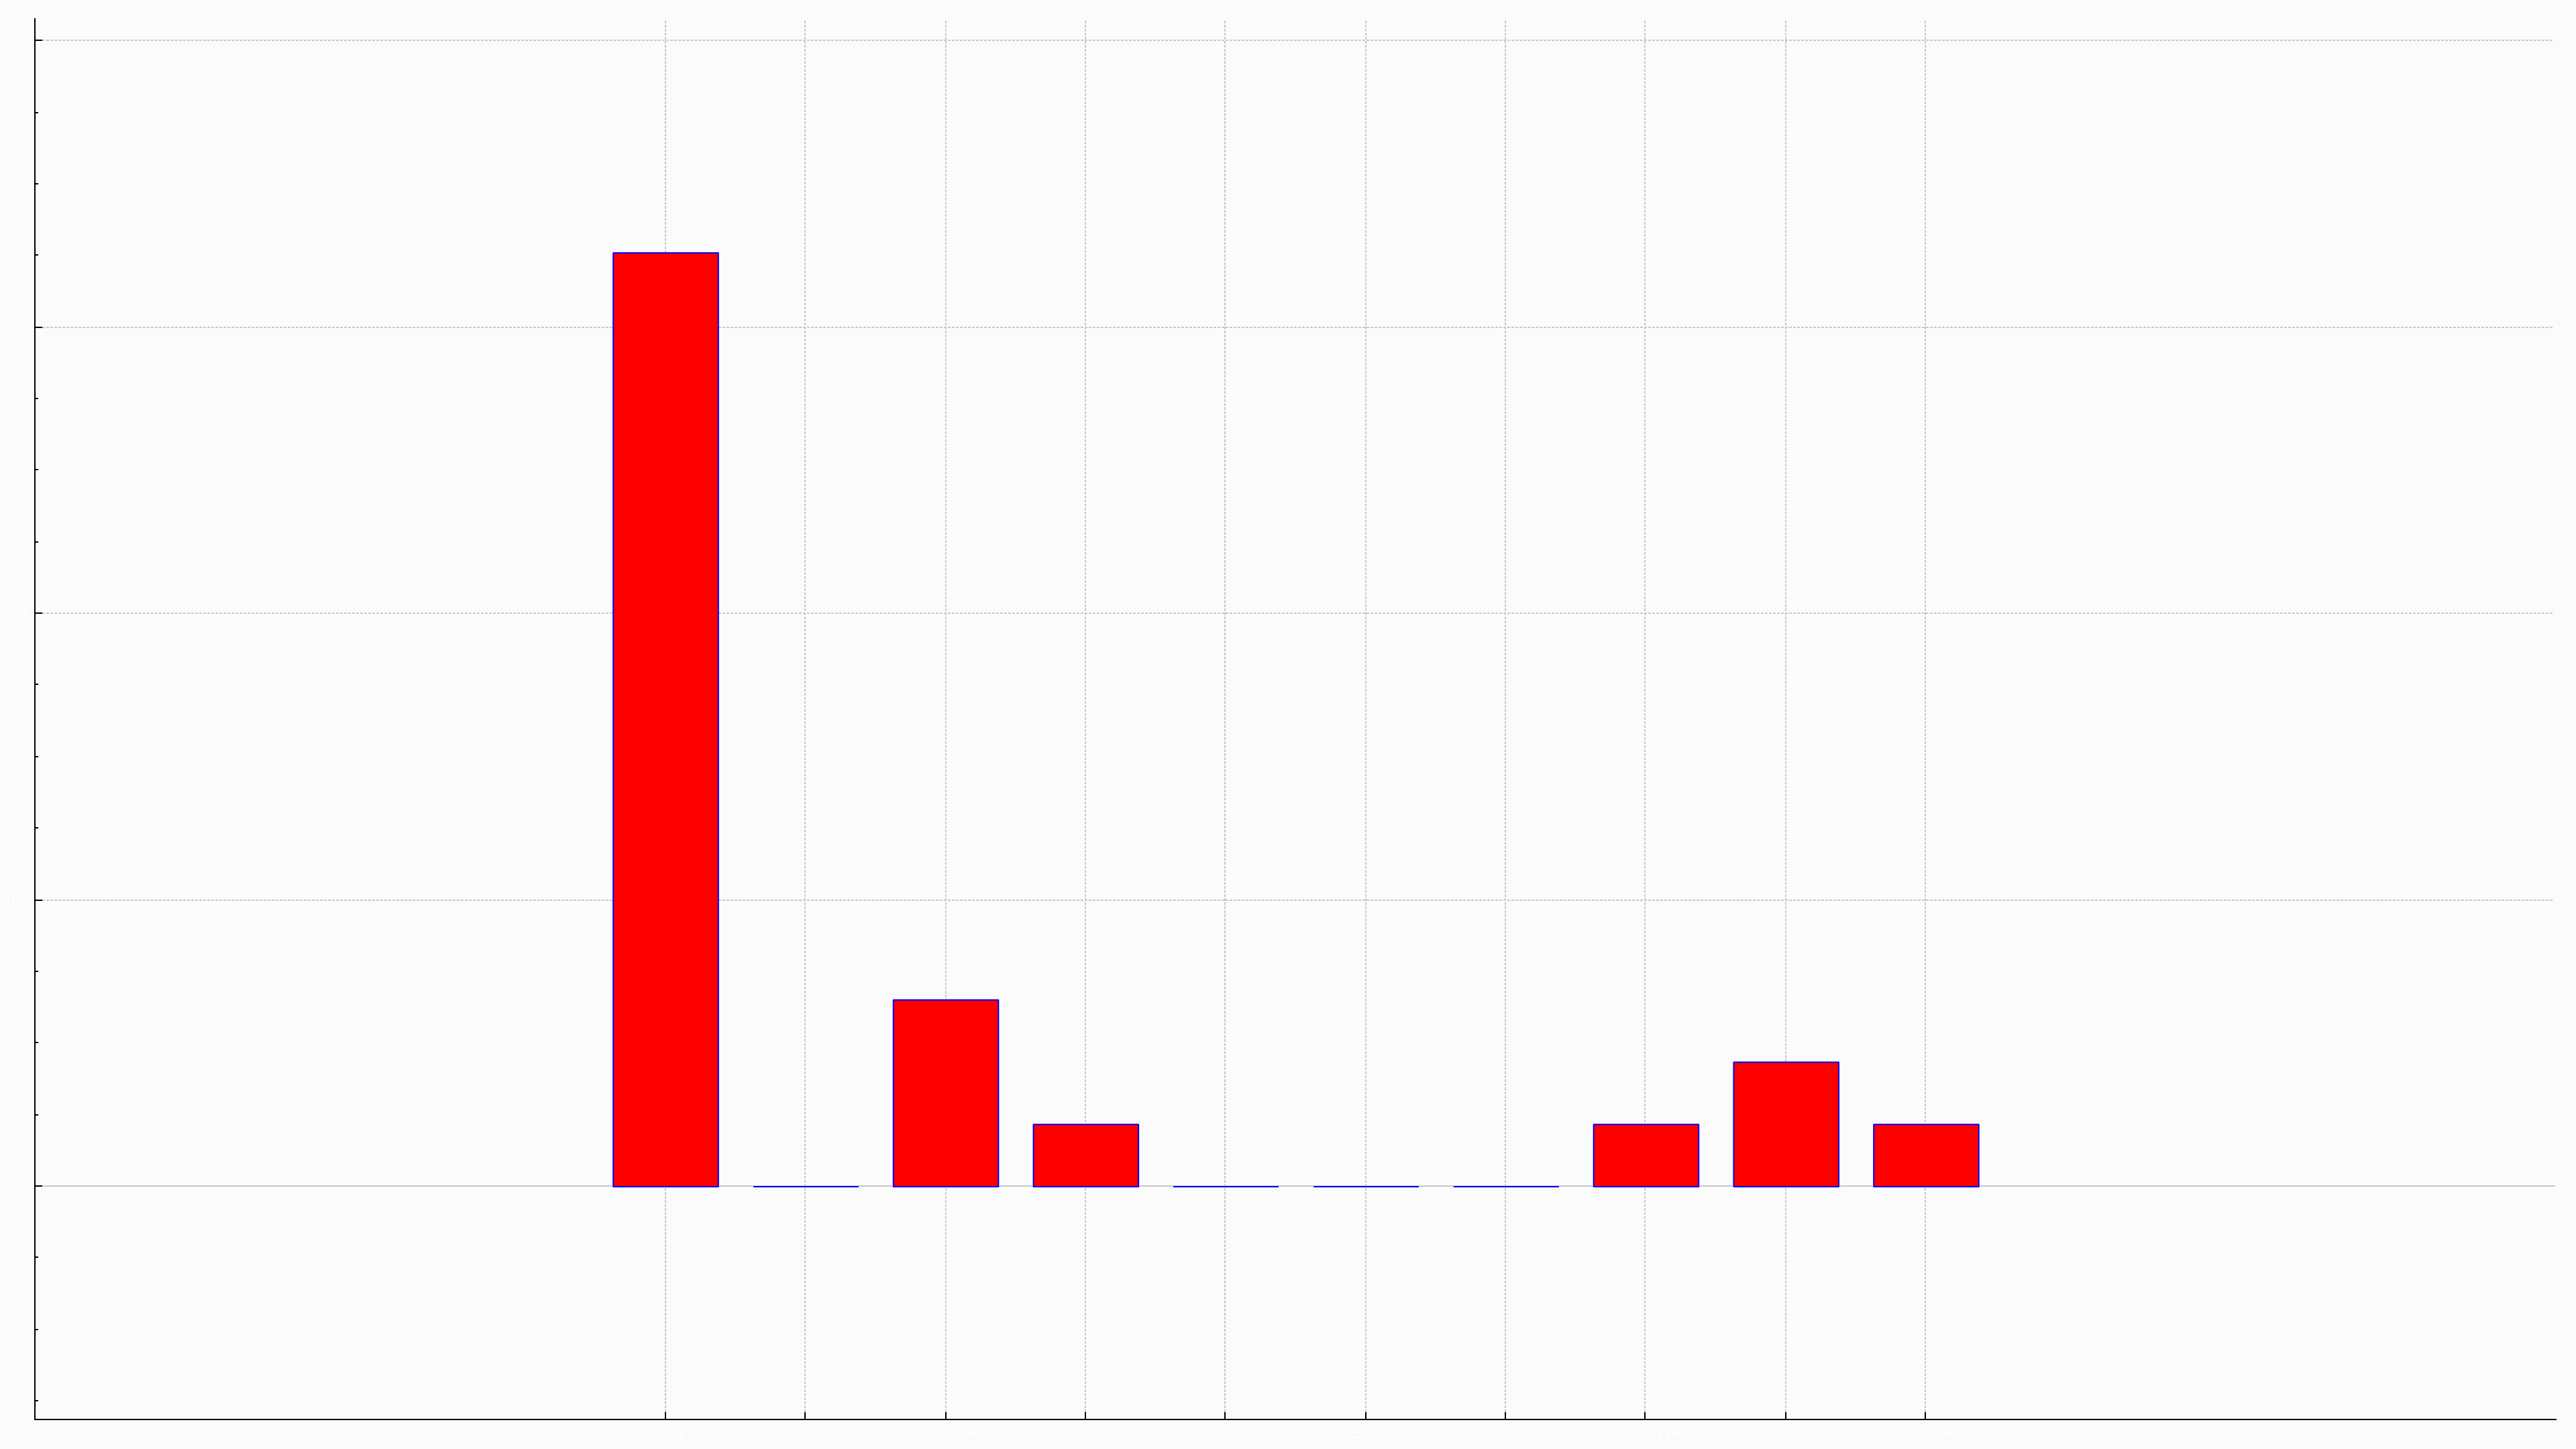
\includegraphics[width=15cm,height = 7.5cm]{charts/hist_cluster_sizePLM.png}}\\
    here the histogram of parallel louvain algorithm, the histogram report the frequency of each bin starting from the lower values terminating with the highests. Two facts are evident from there, first there are more small communities than bigger ones, second there aren't values between bigger and small, meaning that there are only small communities or very bigger ones. 

\end{document}